\documentclass{article} %[a4paper, 10pt, french]

\usepackage[french]{babel}
\usepackage[utf8]{inputenc}
\usepackage[T1]{fontenc}
\usepackage{amsmath,amsfonts,amssymb,mathrsfs}
\frenchbsetup{StandardLists=true}
\usepackage{geometry}
\usepackage{lmodern} %pas pixelisé
\usepackage{engrec,titlesec,lipsum,xcolor}
\usepackage{fancybox}
\usepackage[skins, most]{tcolorbox}
\usepackage[bookmarks={true},bookmarksopen={true}, hidelinks, pdftitle={APP - Fil rouge}, pdfauthor={AAProximation}, pdfsubject={Arbres équilibres AVL}]{hyperref}
\usepackage{setspace}
\usepackage{mathabx}
\usepackage{multicol}
\usepackage{enumitem}
\usepackage{array,multirow,makecell}
\usepackage{titlesec}
\usepackage{multirow}
\usepackage{hyperref}
\usepackage{listings}
\usepackage{graphicx}
\usepackage{caption}
\usepackage{subcaption}
\usepackage{float}

\AddThinSpaceBeforeFootnotes
\FrenchFootnotes
\geometry{hmargin=1.2cm, top=1.2cm, bottom = 1.5cm}
\definecolor{vert}{rgb}{0,0.69,0.31}
\definecolor{bleue}{rgb}{0,0.31,0.69} 
\definecolor{violet}{rgb}{0.38,0.18,055} % 97, 45, 140     244, 208, 63
\definecolor{jaune}{rgb}{0.96, 0.85, 0.23}


\definecolor{darkWhite}{rgb}{0.94,0.94,0.94}
\definecolor{vert}{rgb}{0,0.69,0.31}
\definecolor{rose}{rgb}{1,0.08,0.58}% rgb(255,20,147)
\definecolor{rouge}{rgb}{0.78,0.12,0.08}
\definecolor{bleue}{rgb}{0,0.31,0.69}
\definecolor{gris}{rgb}{0.4,0.4,0.4}
\definecolor{marron}{rgb}{0.4,0.2,0}
\definecolor{darkWhite}{rgb}{0.94,0.94,0.94}

\newtcolorbox{titre}[1][]{enhanced, drop fuzzy shadow southwest, arc=4mm, outer arc=1mm, colback=red!5!white,colframe=red!75!black, boxrule=3pt, center, halign = center, left=1mm, right=1mm,  width = 7.7cm }



\renewcommand*{\lstlistlistingname}{Code Listings}
\renewcommand*{\lstlistingname}{Code Listing}
\definecolor{gray}{gray}{0.5}
\colorlet{commentcolour}{green!50!black}
\colorlet{stringcolour}{red!60!black}
\colorlet{keywordcolour}{magenta!90!black}
\colorlet{exceptioncolour}{yellow!50!red}
\colorlet{commandcolour}{blue!60!black}
\colorlet{numpycolour}{blue!60!green}
\colorlet{literatecolour}{magenta!90!black}
\colorlet{promptcolour}{green!50!black}
\colorlet{specmethodcolour}{violet}


\newcommand*{\framemargin}{3ex}
\newcommand*{\literatecolour}{\textcolor{literatecolour}}
\newcommand*{\pythonprompt}{\textcolor{promptcolour}{{>}{>}{>}}}

 

\definecolor{darkWhite}{rgb}{0.94,0.94,0.94}
 
\lstset{
  aboveskip=3mm,
  belowskip=-2mm,
  backgroundcolor=\color{darkWhite},
  basicstyle=\ttfamily\footnotesize,
  breakatwhitespace=false,
  breaklines=true,
  captionpos=b,
  commentstyle=\color{commentcolour},
  deletekeywords={...},
  emph={[8]spectre, addNode, sortAddNode, Partitionnement_v3, comparer, echanger, strndup, strcspn}, % nom des fonctions
  emphstyle={[8]\color{violet}},
  escapeinside={\%*}{*)},
  extendedchars=true,
  framexleftmargin=16pt,
  framextopmargin=3pt,
  framexbottommargin=6pt,
  %frame=tb,
  frame=trbl,
  keepspaces=true,
  keywordstyle=\color{blue},
  language=C,
  literate=
  {²}{{\textsuperscript{2}}}1
  {⁴}{{\textsuperscript{4}}}1
  {⁶}{{\textsuperscript{6}}}1
  {⁸}{{\textsuperscript{8}}}1
  {€}{{\euro{}}}1
  {é}{{\'e}}1
  {è}{{\`{e}}}1
  {ê}{{\^{e}}}1
  {ë}{{\¨{e}}}1
  {É}{{\'{E}}}1
  {Ê}{{\^{E}}}1
  {û}{{\^{u}}}1
  {ù}{{\`{u}}}1
  {â}{{\^{a}}}1
  {à}{{\`{a}}}1
  {á}{{\'{a}}}1
  {ã}{{\~{a}}}1
  {Á}{{\'{A}}}1
  {Â}{{\^{A}}}1
  {Ã}{{\~{A}}}1
  {ç}{{\c{c}}}1
  {Ç}{{\c{C}}}1
  {õ}{{\~{o}}}1
  {ó}{{\'{o}}}1
  {ô}{{\^{o}}}1
  {Õ}{{\~{O}}}1
  {Ó}{{\'{O}}}1
  {Ô}{{\^{O}}}1
  {î}{{\^{i}}}1
  {Î}{{\^{I}}}1
  {í}{{\'{i}}}1
  {Í}{{\~{Í}}}1,
  morekeywords={*,...},
  numbers=left,
  numbersep=3pt,
  numberstyle=\footnotesize\color{black},
  rulecolor=\color{black},
  showspaces=false,
  showstringspaces=false,
  showtabs=false,
  stepnumber=1,
  stringstyle=\color{orange},
  tabsize=4,
  title=\lstname,
}

 



\title{AAP - Fil Rouge :\\ Compte rendu}
\author{AAProximation \\ Maistret James, Thieffry \'Emile, Chevalier Romain, Feng Yanli \&  Hong Yutong}
\date{\today}

\renewcommand{\thesection}{\arabic{section}}
\newcolumntype{M}{>{\centering\arraybackslash}m{1.5cm}}

\begin{document}
\maketitle
\setcounter{secnumdepth}{3}
\setcounter{tocdepth}{3}

\tableofcontents
\listoffigures

\newpage

\section{Introduction}

Le fil rouge d'AAP 21-22, visait la création d'arbre équilibrés en language C. Le fil rouge consistait à mise en place de trois programmes, le premier permet la création d'une image d'un arbre AVL à partir d'une liste de mot. Quant au second programme, il sert à indexer un dictionnaire dans un arbre AVL dont le tri des mots est basé sur leur signature. Enfin le dernier programme, qui repose sur le second, permet de déterminer les anagrammes d'un mot dans un dictionnaire. 

\section{Programme 1: \texttt{displayAVL.exe}}
\label{sec:prog_1}
\subsection{Développement}
\subsubsection{Fonction de base pour créer l'arbre}
\paragraph{Rotations simples} Le programme de la rotation simple à droite était donné pour la rotation de gauche, nous avons raisonné par analogie et le calcul des facteur de déséquilibre est donné ci-dessous. En se basant sur la figure~\ref{LeftRot}, on a \( a = h(A_g) - h(A_d), b = h(B_g) - h(A)\) et \(h(A) = 1 +\max (h(A_g), h(A_d)) \) où \(h(x)\) est la hauteur du noeud \(x\). Alors 
\begin{align*}
b' &= h(B_g)-h(A_g) \\
&= b + h(A) - h(A_g) & \mathrm{en\  utilisant \ la \  définition \  de } \ b  \\
&= b +  1 +\max (h(A_g), h(A_d)) - h(A_g) & \mathrm{en \ utilisant \ la \ définition\ de} \ h(A)  \\
&= b + 1 + \max(0, h(A_d)-h(A_g))\\
&= b + 1 + \max(0, -a) & \mathrm{en\  utilisant \ la \  définition \  de } \ a \\
&= 1+ b -\min(a,0)
\end{align*} % aime pas les é

Et de même, \( a' = 1 + a + \max(b', 0) \)

\begin{figure}[!h]
\begin{center}
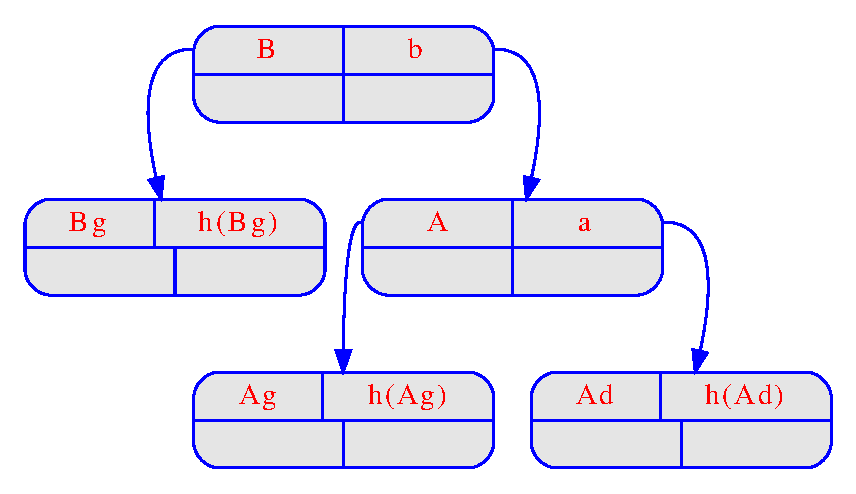
\includegraphics[scale=0.49]{Img_prog1/LeftRotate1.eps}
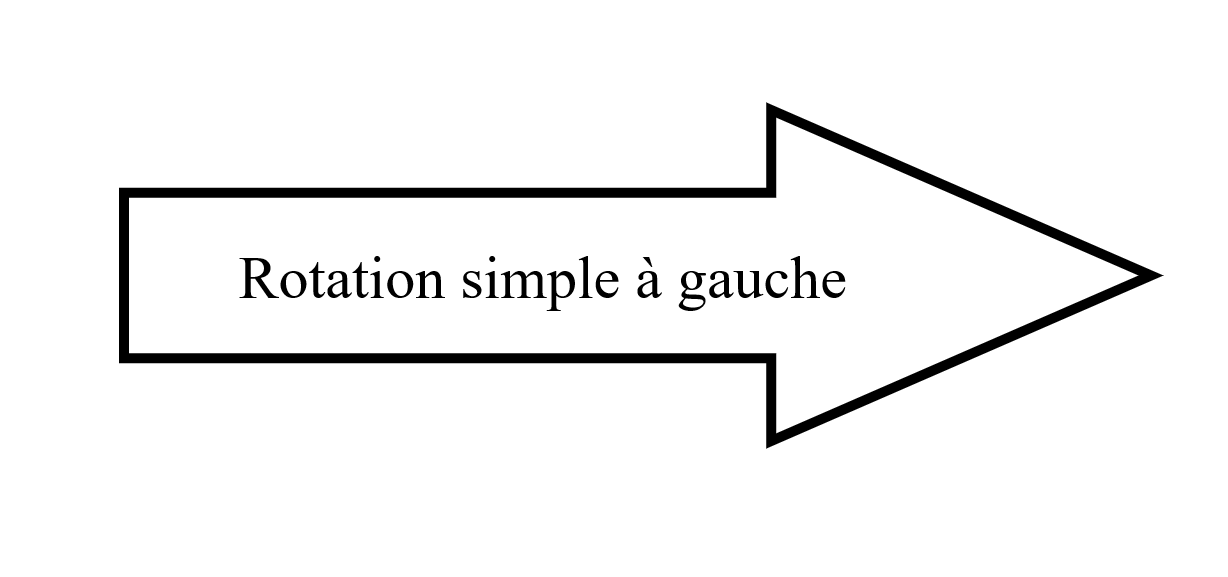
\includegraphics[scale=0.20]{Img_prog1/FlecheLeftrotate.png}
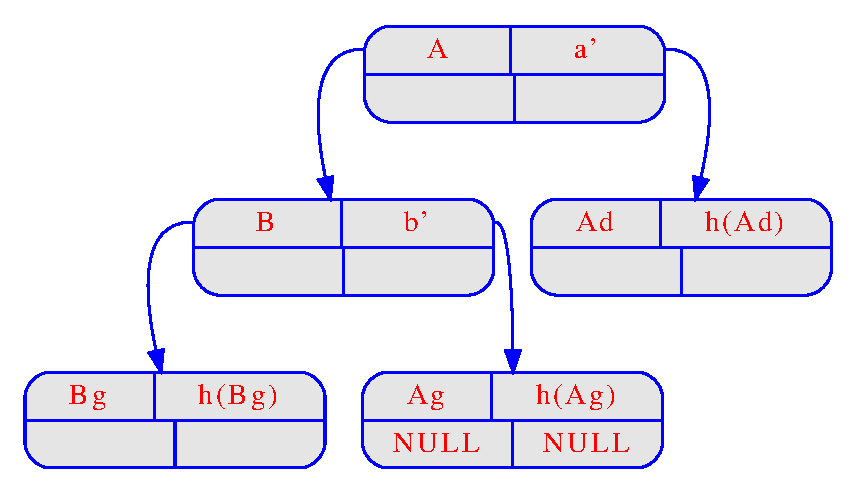
\includegraphics[scale=0.49]{Img_prog1/LeftRotate2.eps}
\end{center}

\caption{Rotation simple à gauche}
\label{LeftRot}
\end{figure}

\paragraph{BalanceAVL} Algorithme donné pour la première partie de la fonction, la seconde partie est l'exacte analogie pour un arbre qui penche de l'autre coté. Lors du développement de cette fonction, nous nous sommes heurté à un problème pour les tests afin de savoir si l'arbre penche, en effet pour faire une rotation double, il faut que le facteur de déséquilibre soit forcément de 2 en valeur absolue et pas seulement non nul, ie l'arbre est bien déséquilibré. Mais une fois rentré dans la rotation double, pour savoir si on fait une rotation double du même coté, ou des deux cotés différents il suffit que l'arbre penche, ie que le facteur de déséquilibre du second nœud a tourner soit non nul. 

% a modifié
\paragraph{InsertAVL} Cette fonction permet d'insérer, au bon endroit, la maille dans l'arbre AVL. Pour cela, on s'est basé sur l'algorithme donné en séance 5 que nous avons traduit en C.

\paragraph{FreeAVL} Cette fonction permet de libérer la mémoire occupé par l'arbre à la fin de l'exécution. Pour cela, elle repose sur la fonction \texttt{free}. 

\subsubsection{Lecture du fichier}
En se basant sur \cite{lect_lines}, nous lisons ligne par ligne le fichier, car il y a un mot par ligne dans le fichier, en ajoutant un compteur de lignes lues afin de respecter le nombre de mots à mettre dans l'arbre renseigné par l'utilisateur.  

\subsubsection{Affichage avec graphviz}
Les fonctions permettant de générer le fichier \texttt{.dot} étaient déjà données, néanmoins le programme ne prenait en compte les noms composés (ie les noms avec un tiret dedans). Afin de corriger cette erreur, il a fallut ajouter des guillemets (donc la séquence suivant \texttt{\textbackslash "\%s\textbackslash "}) dans les noms des blocs graphviz à afficher. De plus, l'affichage du facteur de déséquilibre n'était pas configuré, nous l'avons donc ajouté à coté du nom de famille du nœud.



\subsection{Jeux de test, exemples d'exécution}
On trouve en figure~\ref{fig:prog1_1} , les différentes étapes de construction de l'arbre pour 10 premiers mots du fichier \texttt{PrenomsV2.txt}. Un exemple d'arbre à 20 mots du fichier \texttt{PrenomsV1.txt} en figure~\ref{fig:prog1_2}.

\begin{figure}[p]
  
  \begin{center}
    \rule{\linewidth}{.5pt}
    \subcaptionbox{Etape 1}{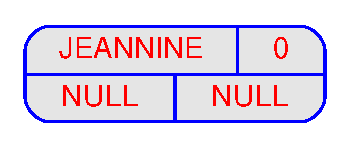
\includegraphics[scale=0.6]{Img_prog1/displayAVL_v00.eps}} \vline
    \subcaptionbox{Etape 2}{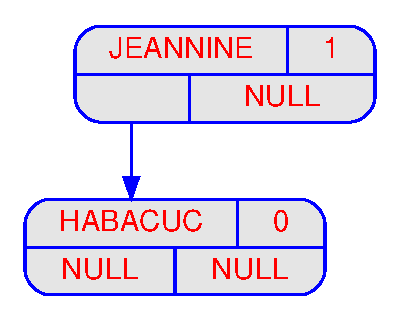
\includegraphics[scale=0.6]{Img_prog1/displayAVL_v01.eps}} \vline
    \subcaptionbox{Etape 3}{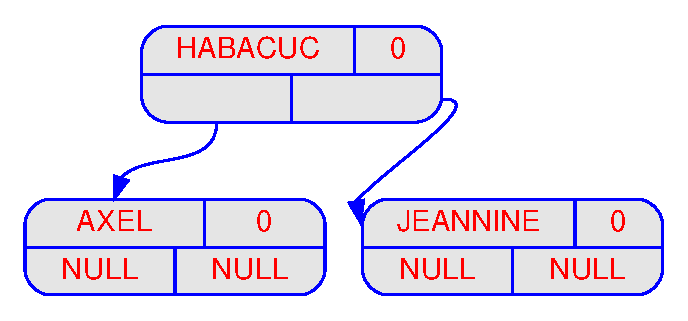
\includegraphics[scale=0.6]{Img_prog1/displayAVL_v02.eps}} \rule{\linewidth}{.5pt} %\vline
    \subcaptionbox{Etape 4}{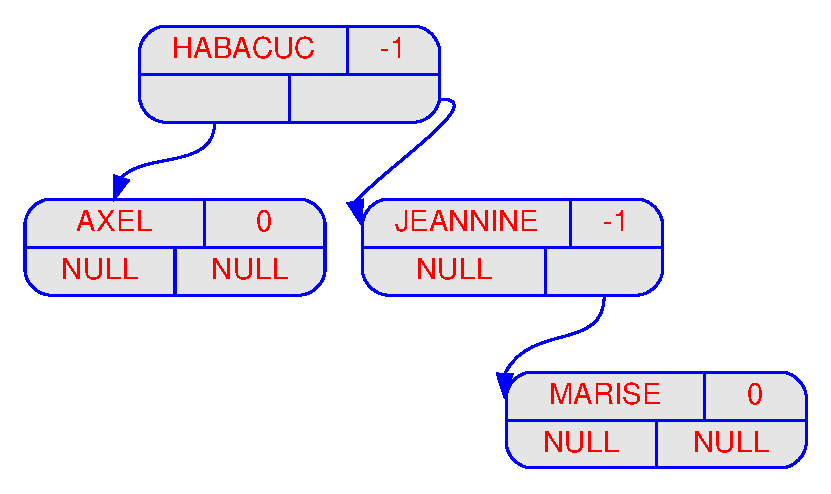
\includegraphics[scale=0.4]{Img_prog1/displayAVL_v03.eps}} \vline
    \subcaptionbox{Etape 5}{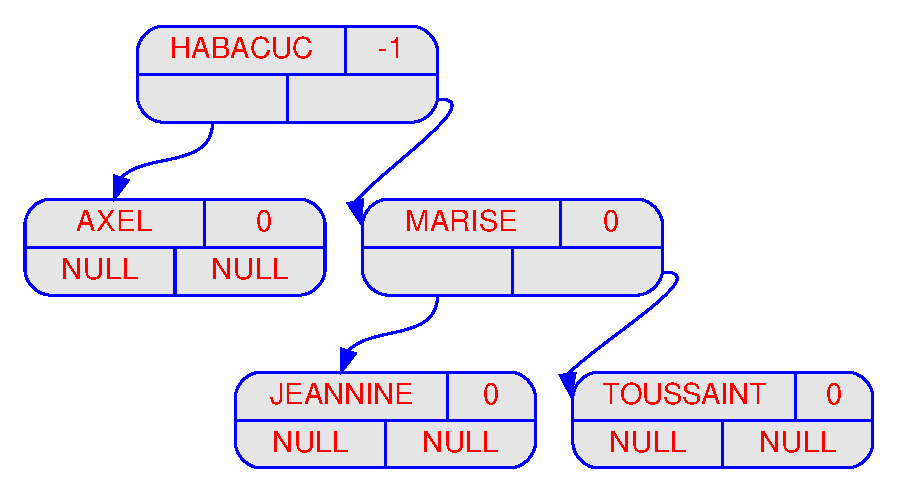
\includegraphics[scale=0.4]{Img_prog1/displayAVL_v04.eps}} \vline
    \subcaptionbox{Etape 6}{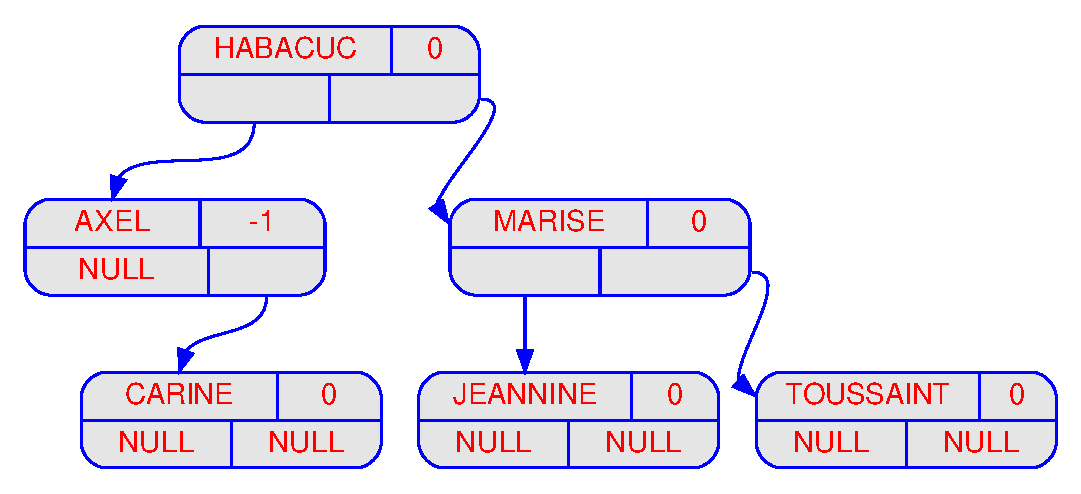
\includegraphics[scale=0.4]{Img_prog1/displayAVL_v05.eps}} \rule{\linewidth}{.5pt} %\vline
    \subcaptionbox{Etape 7}{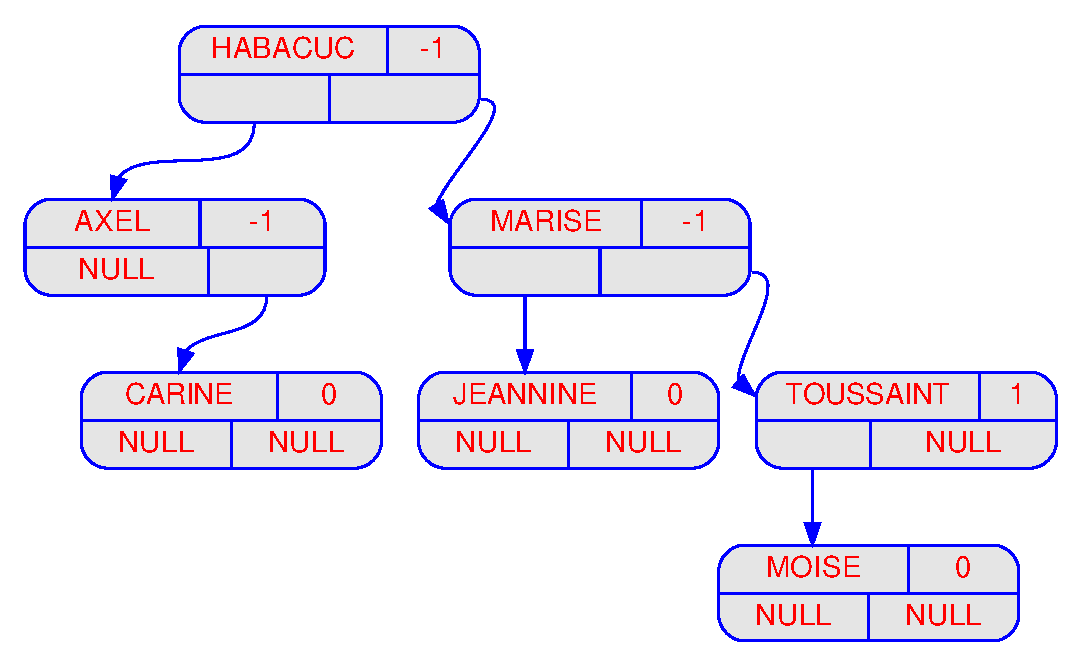
\includegraphics[scale=0.45]{Img_prog1/displayAVL_v06.eps}} \vline
    \subcaptionbox{Etape 8}{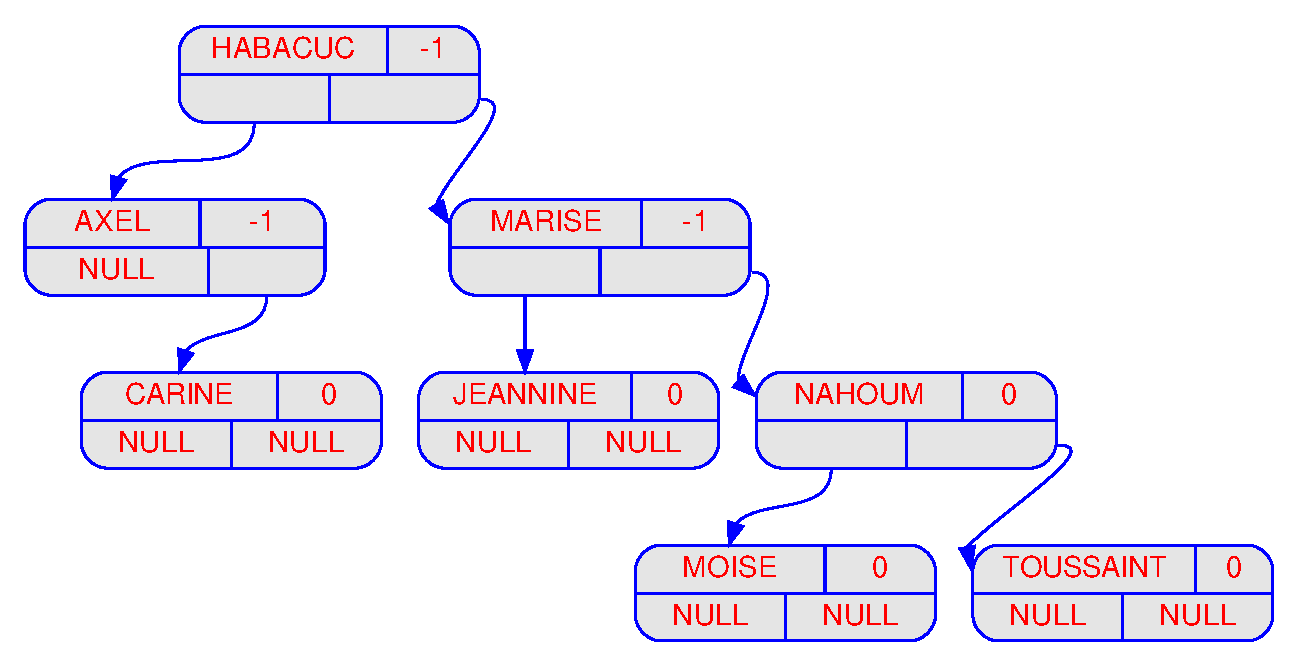
\includegraphics[scale=0.45]{Img_prog1/displayAVL_v07.eps}} \rule{\linewidth}{.5pt} %\vline
    \subcaptionbox{Etape 9}{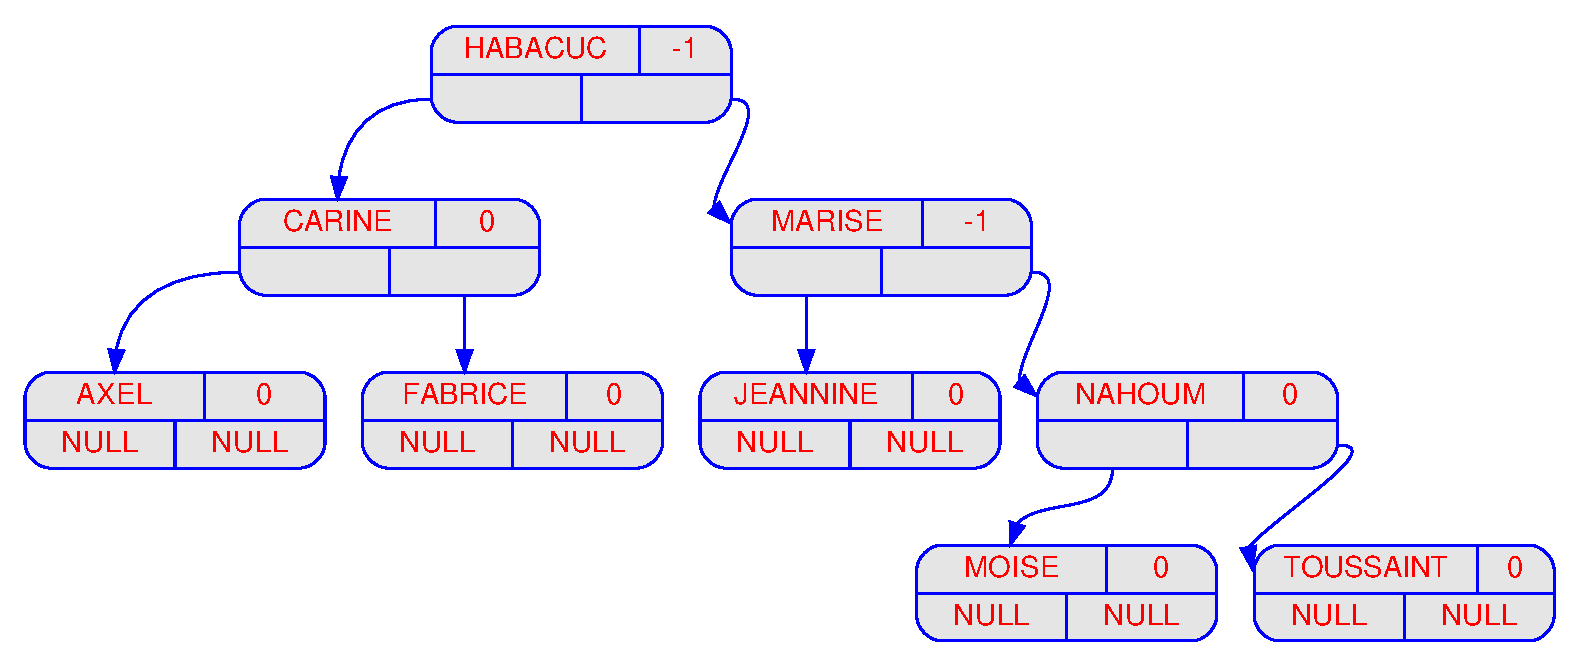
\includegraphics[scale=0.35]{Img_prog1/displayAVL_v08.eps}} \vline
    \subcaptionbox{Etape 10}{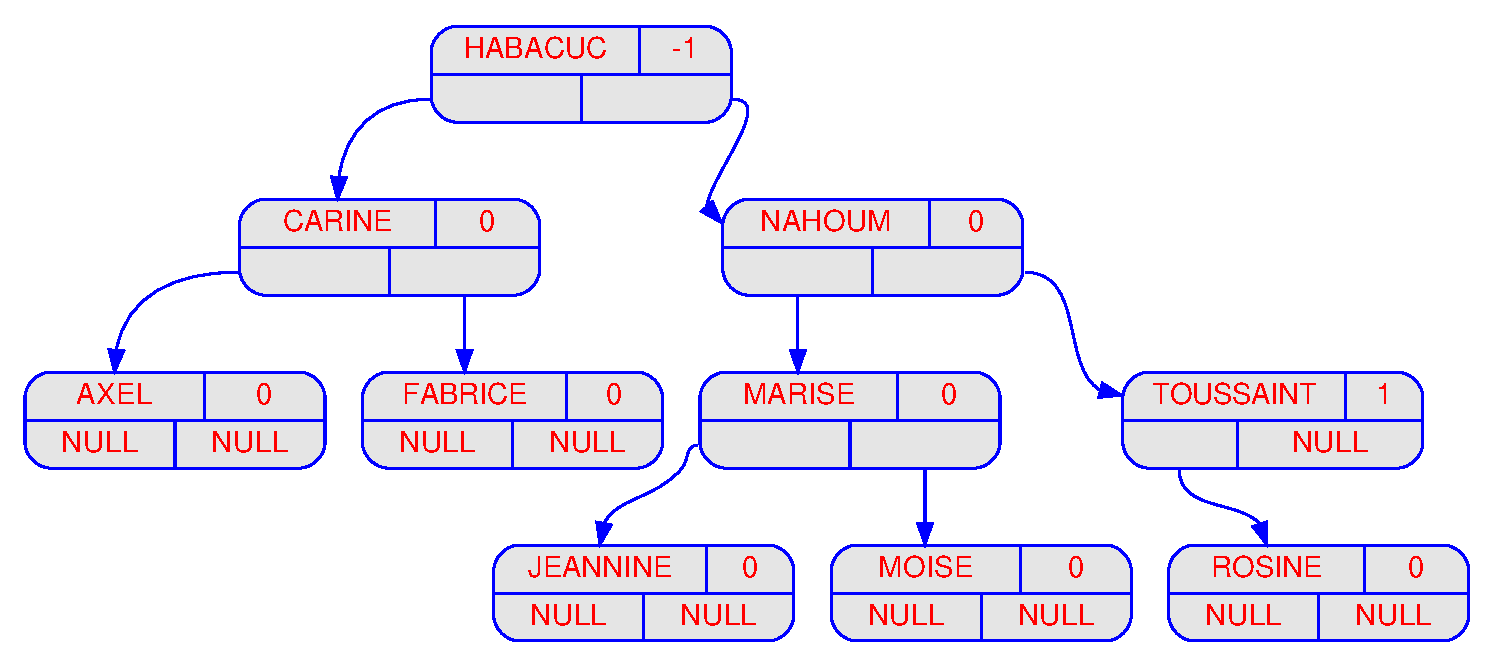
\includegraphics[scale=0.35]{Img_prog1/displayAVL_v09.eps}}  \rule{\linewidth}{.5pt} %\vline
   
    
  \end{center}
  
  \caption{Construction de l'arbre pour les 10 premiers prénoms de \texttt{PrenomsV2.txt}}
  \label{fig:prog1_1}
\end{figure}

\begin{figure}[p]
  \begin{center}
    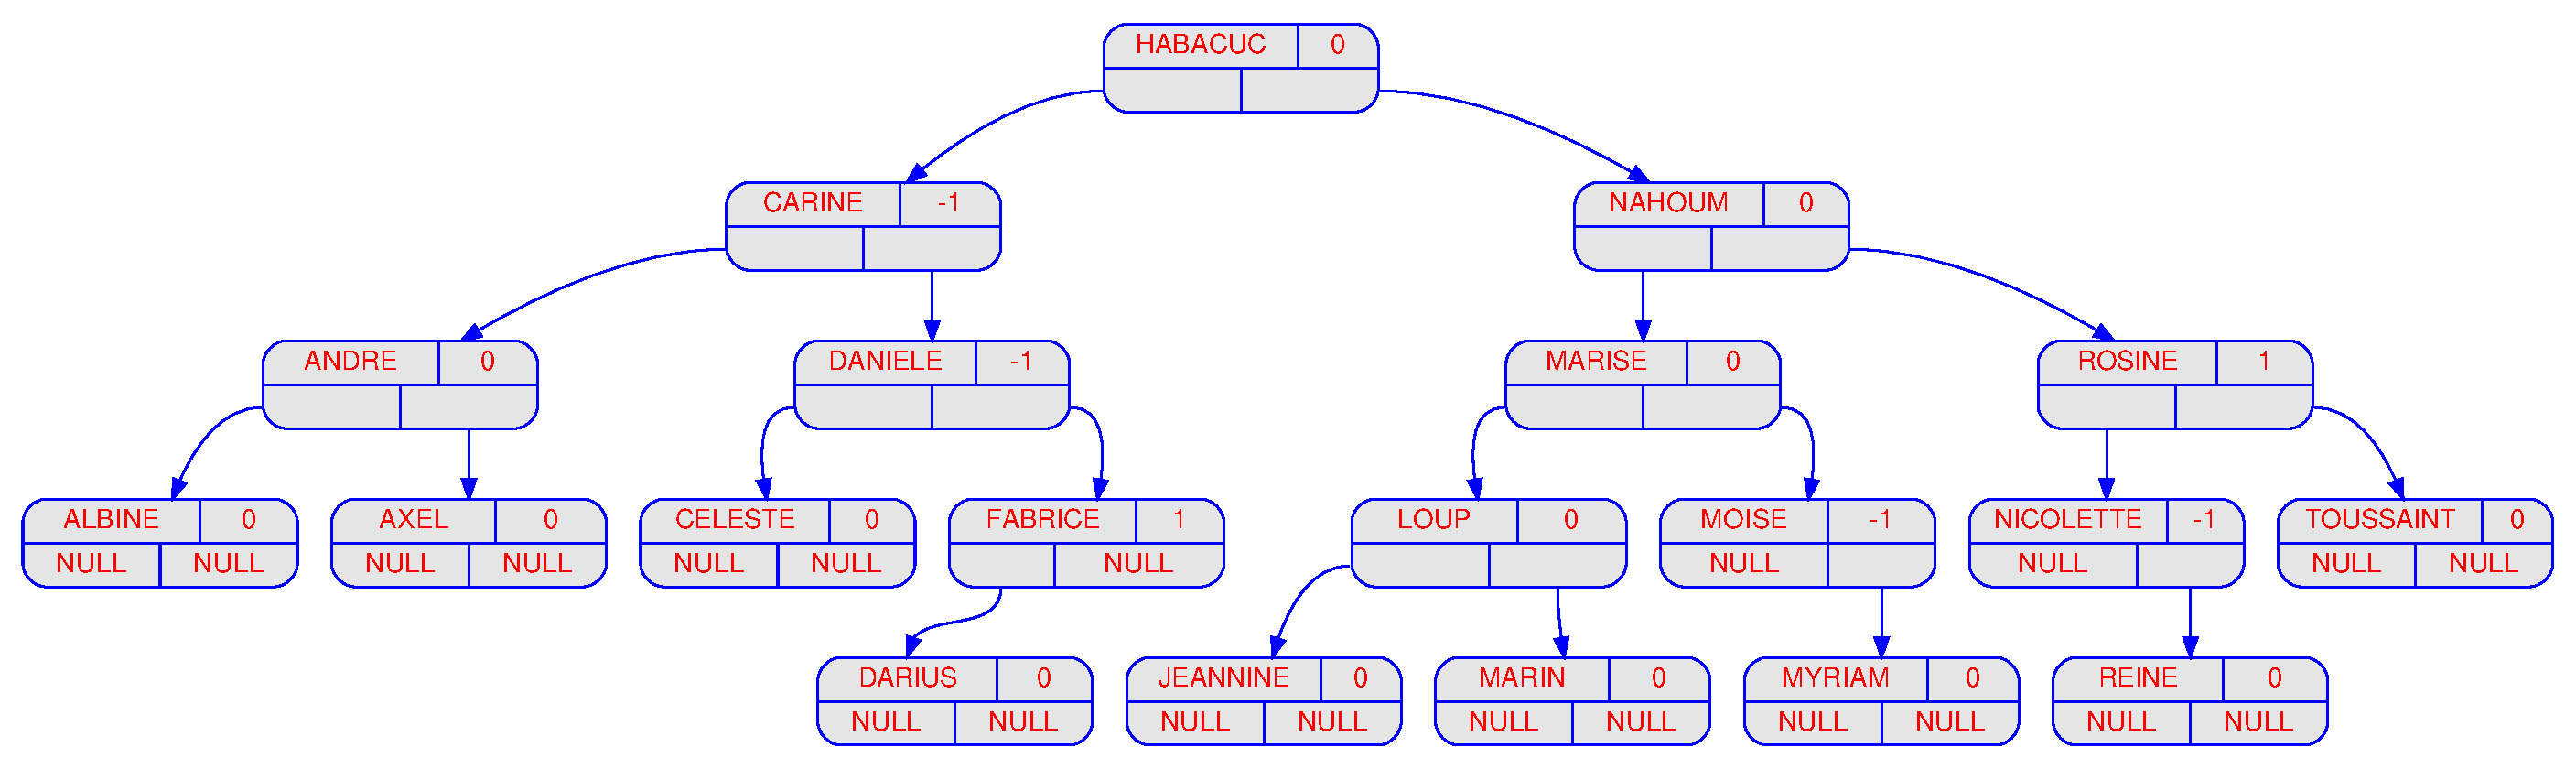
\includegraphics[scale=0.36]{Img_prog1/displayAVL_20.eps}
  \end{center}
  \caption{Exemple arbre avec les 20 premiers prénoms de \texttt{PrenomsV1.txt}}
  \label{fig:prog1_2}
\end{figure}

\section{Programme 2: \texttt{indexation.exe} \label{sec:prog_2}}
\subsection{Développement}

\subsubsection{Fonction de base pour créer l'arbre}
\paragraph{Restructuration des mailles} Pour ce programme, nous avons rajouté un champ dans chaque maille de l'arbre. Dans un premier temps, nous avons décidé que le champ \texttt{T\_avl NodeAVL->val} deviendrai la signature des mots contenus dans le nouveau champ \texttt{T\_avl NodeAVL->list\_mots} qui contient la liste de tout les mots comportant la même signature. Voir illustration des champs d'une maille en figure~\ref{fig:champs_maille} et un exemple en figure~\ref{fig:exemple:maille}.

\begin{figure}[H]
  \begin{center}
    \subcaptionbox{Champs de la maille\label{fig:champs_maille}}{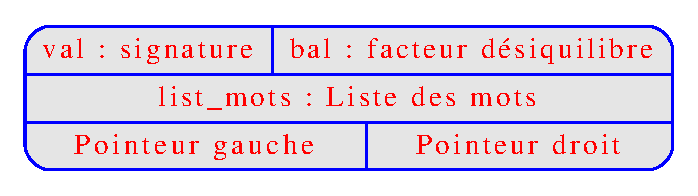
\includegraphics[scale=0.75]{Img_prog2/Maille_vide.eps}}
    \subcaptionbox{Exemple de maille\label{fig:exemple:maille}}{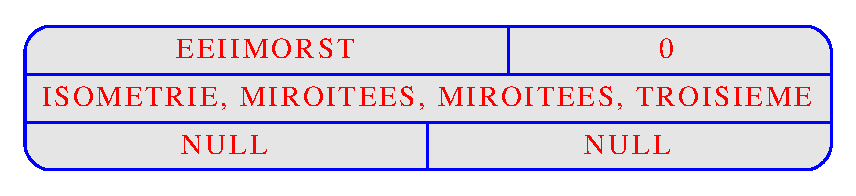
\includegraphics[scale=0.75]{Img_prog2/Maille_exemple.eps}}
  \end{center}
  \caption{Restructuration des mailles pour le second programme}
  \label{fig:restruc_pro2}
\end{figure}

\paragraph{Calcul de la signature} Pour calculer la signature d'un mot, on trie les lettres de ce mot. Dans un premier temps, nous avions utilisé les fonctions de tri fusion du TEA de la semaine 3. Et comme dans ce TEA, nous avions remarqué que le temps de tri de la fonction \texttt{qsort} était beaucoup plus faible que le temps du tri fusion. Finalement, nous utilisons la fonction \texttt{qsort} pour trier les lettres et donc calculer la signature. 

\paragraph{Ajout de mot dans un arbre déjà construit} Pour ajouter un mot dans un arbre AVL déjà construit, deux cas de figure se présente: \begin{itemize}
  \item Il n'y a pas de maille avec la signature de ce mot, dans ce cas, on crée une nouvelle maille avec la signature de ce mot et ce mot et on l'ajoute au bon endroit, en suivant le même algorithme que dans le programme 1 (cf. \ref{sec:prog_1} - \texttt{displayAVL.exe}). Dont la comparaison entre les mailles se fait sur la signature. 
  \item Si il y a déjà une maille avec la signature du mot à ajouter, on ajoute le mot au champ \texttt{list\_mots}, en prenant garde de réallouer de la mémoire à ce champ et en concaténant le champ \texttt{list\_mots} et le mot grâce à la fonction \texttt{strcat} de la librairie \texttt{string.h}.
\end{itemize}

\paragraph{Remarque} On récupère le taille des mots dès la première ligne du fichier ouvert, et on le met en argument de chaque fonction afin de ne pas avoir à le recalculer et ainsi gagner du temps de calcul. 

\subsubsection{Calcul des paramètres de l'arbre}
Pour calculer le nombre de noeud et la hauteur de l'arbre, on utilise la fonction \texttt{nbNodesAVL} et \texttt{heightAVL}, donnée lors de la séance 4. Pour compter le nombre de mots, noté \(N\) , on incrémente un compteur à mot qu'on ajoute à l'arbre. La taille des mots est récupéré dès l'ouverture du ficher grâce à la fonction \texttt{strlen}. Pour la durée, on fait la différence entre les heures de début et de fin de la construction. Et enfin pour calculer la hauteur minimale d’un arbre contenant le même nombre de noeud, on calcul \(\displaystyle \max \left\lbrace k \in \mathbb{N}, \quad 0 < \left\lfloor  \frac{N}{2^k} \right\rfloor  \right\rbrace \), ce qui correspond à \(\left\lceil \log_2 (N) \right\rceil \). 

\subsubsection{Recherche de mots}

\paragraph{Recherche d'un mot}Pour rechercher si un mot est présent dans l'arbre, on récupère le mot entré au clavier par l'utilisateur grâce à la fonction \texttt{fgets}, avec l'argument \texttt{stdin}, en faisant bien attention de supprimer le retour chariot \texttt{\textbackslash n} qui s'ajoute au mot écrit par l'utilisateur à l'aide de la commande en figure~\ref{fig:recherche_mot}. Ensuite, on recherche le mot grâce à la fonction \texttt{searchAVL\_rec} donnée en séance 4. 

\begin{figure}[H]
  \begin{lstlisting}
    fgets(mot_ecris, 27, stdin) // 27 correspond au nombre maximum de caractères entré par l'utilisateur   (mot le plus long de la langue française à 26 caractères)
    mot_cherche = strndup(mot_ecris, strcspn(mot_ecris, "\n"));
    // la variable mot_ecris correspond au mot entré par l'utilisateur \end{lstlisting}
  
    \caption{Récupération mot entré par l'utilisateur pour la recherche dans l'arbre}
    \label{fig:recherche_mot}
\end{figure}


\paragraph{Profondeur du noeud} Pour calculer la profondeur, on compte le nombre de fois où l'on fait appel à la fonction récursive \texttt{searchAVL\_rec}, pour cela on passe ce compteur en argument de la fonction de recherche. 

\subsection{Jeux de test, exemples d'exécution}
On trouve en figure~\ref{fig:prog_2} la sortie du programme \texttt{indexation.exe} pour le dictionnaire \texttt{Dico\_09.txt}.

\begin{figure}[H]
  \begin{lstlisting}
    Taille des mots : 9
    Nombre de mots: 70039
    Durée de construction: 273.47 
    Nombre de noeuds: 43444
    Hauteur: 18
    Hauteur minimale d un arbre contenant 43444 noeuds: 16
    Entrer le mot à rechercher (Ctrl+D) pour terminer: RENIPPEES
    RENIPPEES
    Profondeur: 17
    Temps de recherche: 0.03
    Entrer le mot à rechercher (Ctrl+D) pour terminer: DECHARNEE
    ADHERENCE, ADHERENCE, DECHARNEE, DECHARNEE
    Profondeur: 9
    Temps de recherche: 0.02
    Entrer le mot à rechercher (Ctrl+D) pour terminer: mot
    Mot non trouvé
    Entrer le mot à rechercher (Ctrl+D) pour terminer: // Ctrl+D entré \end{lstlisting}
    \caption{Execution \texttt{indexation.exe} avec dictionnaire \texttt{Dico\_09.txt}}
    \label{fig:prog_2}
\end{figure}


\section{Programme 3: \texttt{anagrammes.exe}}
\subsection{Développement}
Pour construire l'arbre, on procède comme dans le programme 2 \texttt{indexation.exe} (cf. \ref{sec:prog_2})

\paragraph{Nombre anagrammes} Pour compter le nombre d'anagrammes, on utilise la fonction \texttt{nb\_anagrammes}, voir en figure~\ref{fig:nb_anag}. Pour cela, on parcourt tout l'arbre récursivement et on compte le nombre de fois où le champ \texttt{list\_mots} (cf. \ref{fig:champs_maille}) possède plus de caractères que un mot seul. 

\paragraph{Affichage des anagrammes} Afin d'afficher les anagrammes, lorsqu'on les compte dans la fonction \texttt{nb\_anagrammes} on ajoute les anagrammes à un fichier externe afin de garder seulement ce qui nous intéresse de l'arbre (cf. ligne 7 en figure~\ref{fig:nb_anag}). Puis à partir de ce fichier, on crée une liste chaînée, grâce aux fonctions développées en TEA, dont chaque maille contient la liste anagrammes d'une même signature. Pour finir, on trie la liste chaînée en fonction de la longueur de la liste de mots contenue dans chaque maille, par ordre décroissant. 

\begin{figure}[H]
  \begin{lstlisting}
int nb_anagramme(T_avl root, int taille_mots, FILE *fp){
  int compteur = 0; // Vaut 0 si pas d'anagramme pour cette maille et 1 si il y a des anagrammes

  if (root!=NULL){
    if (strlen(root->list_mots)>taille_mots){ // On regarde si la liste de mots de maille contient plus d'un mot
      compteur++; //Si c'est le cas, c'est que c'est qu'il y a des anagrammes de ce mot
            fprintf(fp, "%s\n", root->list_mots); // On ajoute les anagrammes au fichier de stockage
    }

    return compteur + nb_anagramme(root->l, taille_mots, fp) + nb_anagramme(root->r, taille_mots, fp); // Compte le nombre de mots du dictionnaire disposant d anagrammes
  }

  return 0;
}\end{lstlisting}
\caption{Fonction: \texttt{nb\_anagrammes}, programme 3}
\label{fig:nb_anag}
  
\end{figure}

\subsection{Jeux de test, exemples d'exécution}

On trouve en figure~\ref{fig:prog_3_2} , la liste chaînée triée par ordre décroissant pour le dictionnaire \texttt{Dico\_16.txt} et en figure~\ref{fig:prog_3_1} la sortie du programme \texttt{anagramme.exe} pour ce même dictionnaire.

\begin{figure}[H]
  \begin{center}
    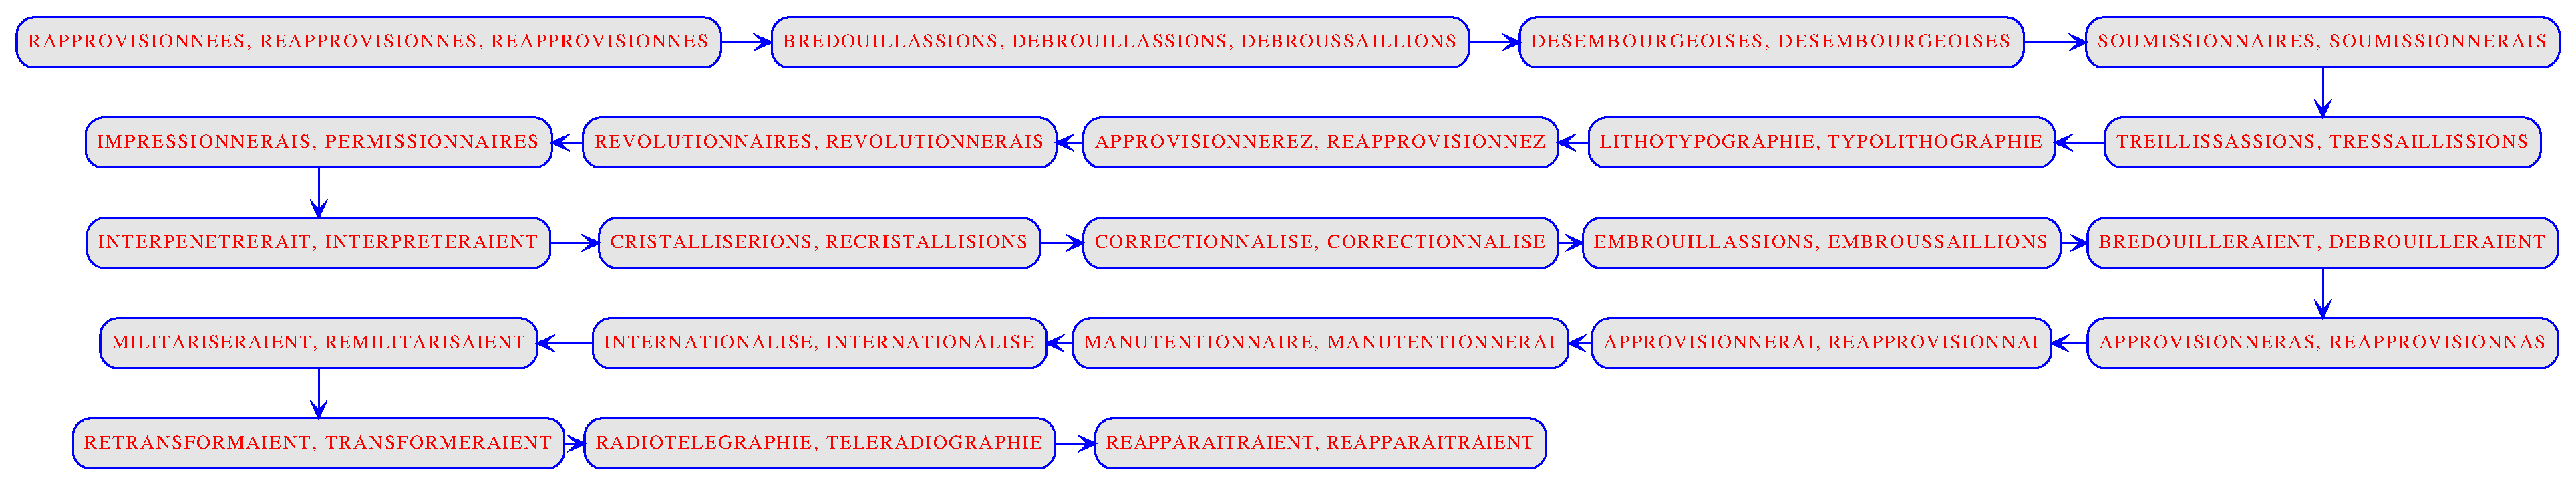
\includegraphics[scale=0.28]{Img_prog3/liste_chaine.eps}
  \end{center}
  \caption{Liste chaînée des anagrammes pour le dictionnaire \texttt{Dico\_16.txt}}
  \label{fig:prog_3_2}
\end{figure}

\begin{figure}[H]
  \begin{lstlisting}
Nombre anagrammes: 22
Listes anagrammes:
RAPPROVISIONNEES, REAPPROVISIONNES, REAPPROVISIONNES
BREDOUILLASSIONS, DEBROUILLASSIONS, DEBROUSSAILLIONS
DESEMBOURGEOISES, DESEMBOURGEOISES
SOUMISSIONNAIRES, SOUMISSIONNERAIS
TREILLISSASSIONS, TRESSAILLISSIONS
LITHOTYPOGRAPHIE, TYPOLITHOGRAPHIE
APPROVISIONNEREZ, REAPPROVISIONNEZ
REVOLUTIONNAIRES, REVOLUTIONNERAIS
IMPRESSIONNERAIS, PERMISSIONNAIRES
INTERPENETRERAIT, INTERPRETERAIENT
CRISTALLISERIONS, RECRISTALLISIONS
CORRECTIONNALISE, CORRECTIONNALISE
EMBROUILLASSIONS, EMBROUSSAILLIONS
BREDOUILLERAIENT, DEBROUILLERAIENT
APPROVISIONNERAS, REAPPROVISIONNAS
APPROVISIONNERAI, REAPPROVISIONNAI
MANUTENTIONNAIRE, MANUTENTIONNERAI
INTERNATIONALISE, INTERNATIONALISE
MILITARISERAIENT, REMILITARISAIENT
RETRANSFORMAIENT, TRANSFORMERAIENT
RADIOTELEGRAPHIE, TELERADIOGRAPHIE
REAPPARAITRAIENT, REAPPARAITRAIENT\end{lstlisting}
\caption{Execution \texttt{anagrammes.exe} avec dictionnaire \texttt{Dico\_16.txt}}
\label{fig:prog_3_1}
\end{figure}



\section{Gestion de projet} Dans un premier temps, nous avons tous bien lu le sujet et bien compris les enjeux. Nous avons alors utilisé les séances 4 et 5 pour decomposer le projet en différentes lot (dont on retrouve la décomposition en figure~\ref{fig:WBS}), de se répartir les tâches et commencer le projet tous ensemble. La répartition des tâches se trouve sur la matrice RACI en figure~\ref{fig:RACI} .Cela nous a permis de finir les 2 premiers programmes rapidement. Nous avons aussi été aidé par M. Slim Hammadi, notamment lorsque nous étions bloqué au programme 2, sur la comprehension du sujet d’un point technique. Nous ne comprenions pas exactement ce qu’il fallait mettre dans les maille de l'arbre (entre autres la liste des mots regroupés par signature). Nous avons chacun fini nos tâches à faire pour la rentrée et nous avons alors pu faire une mise en commun de travail et vérifier que tout fonctionne correctement.


\begin{figure}[H]
  \begin{center}
    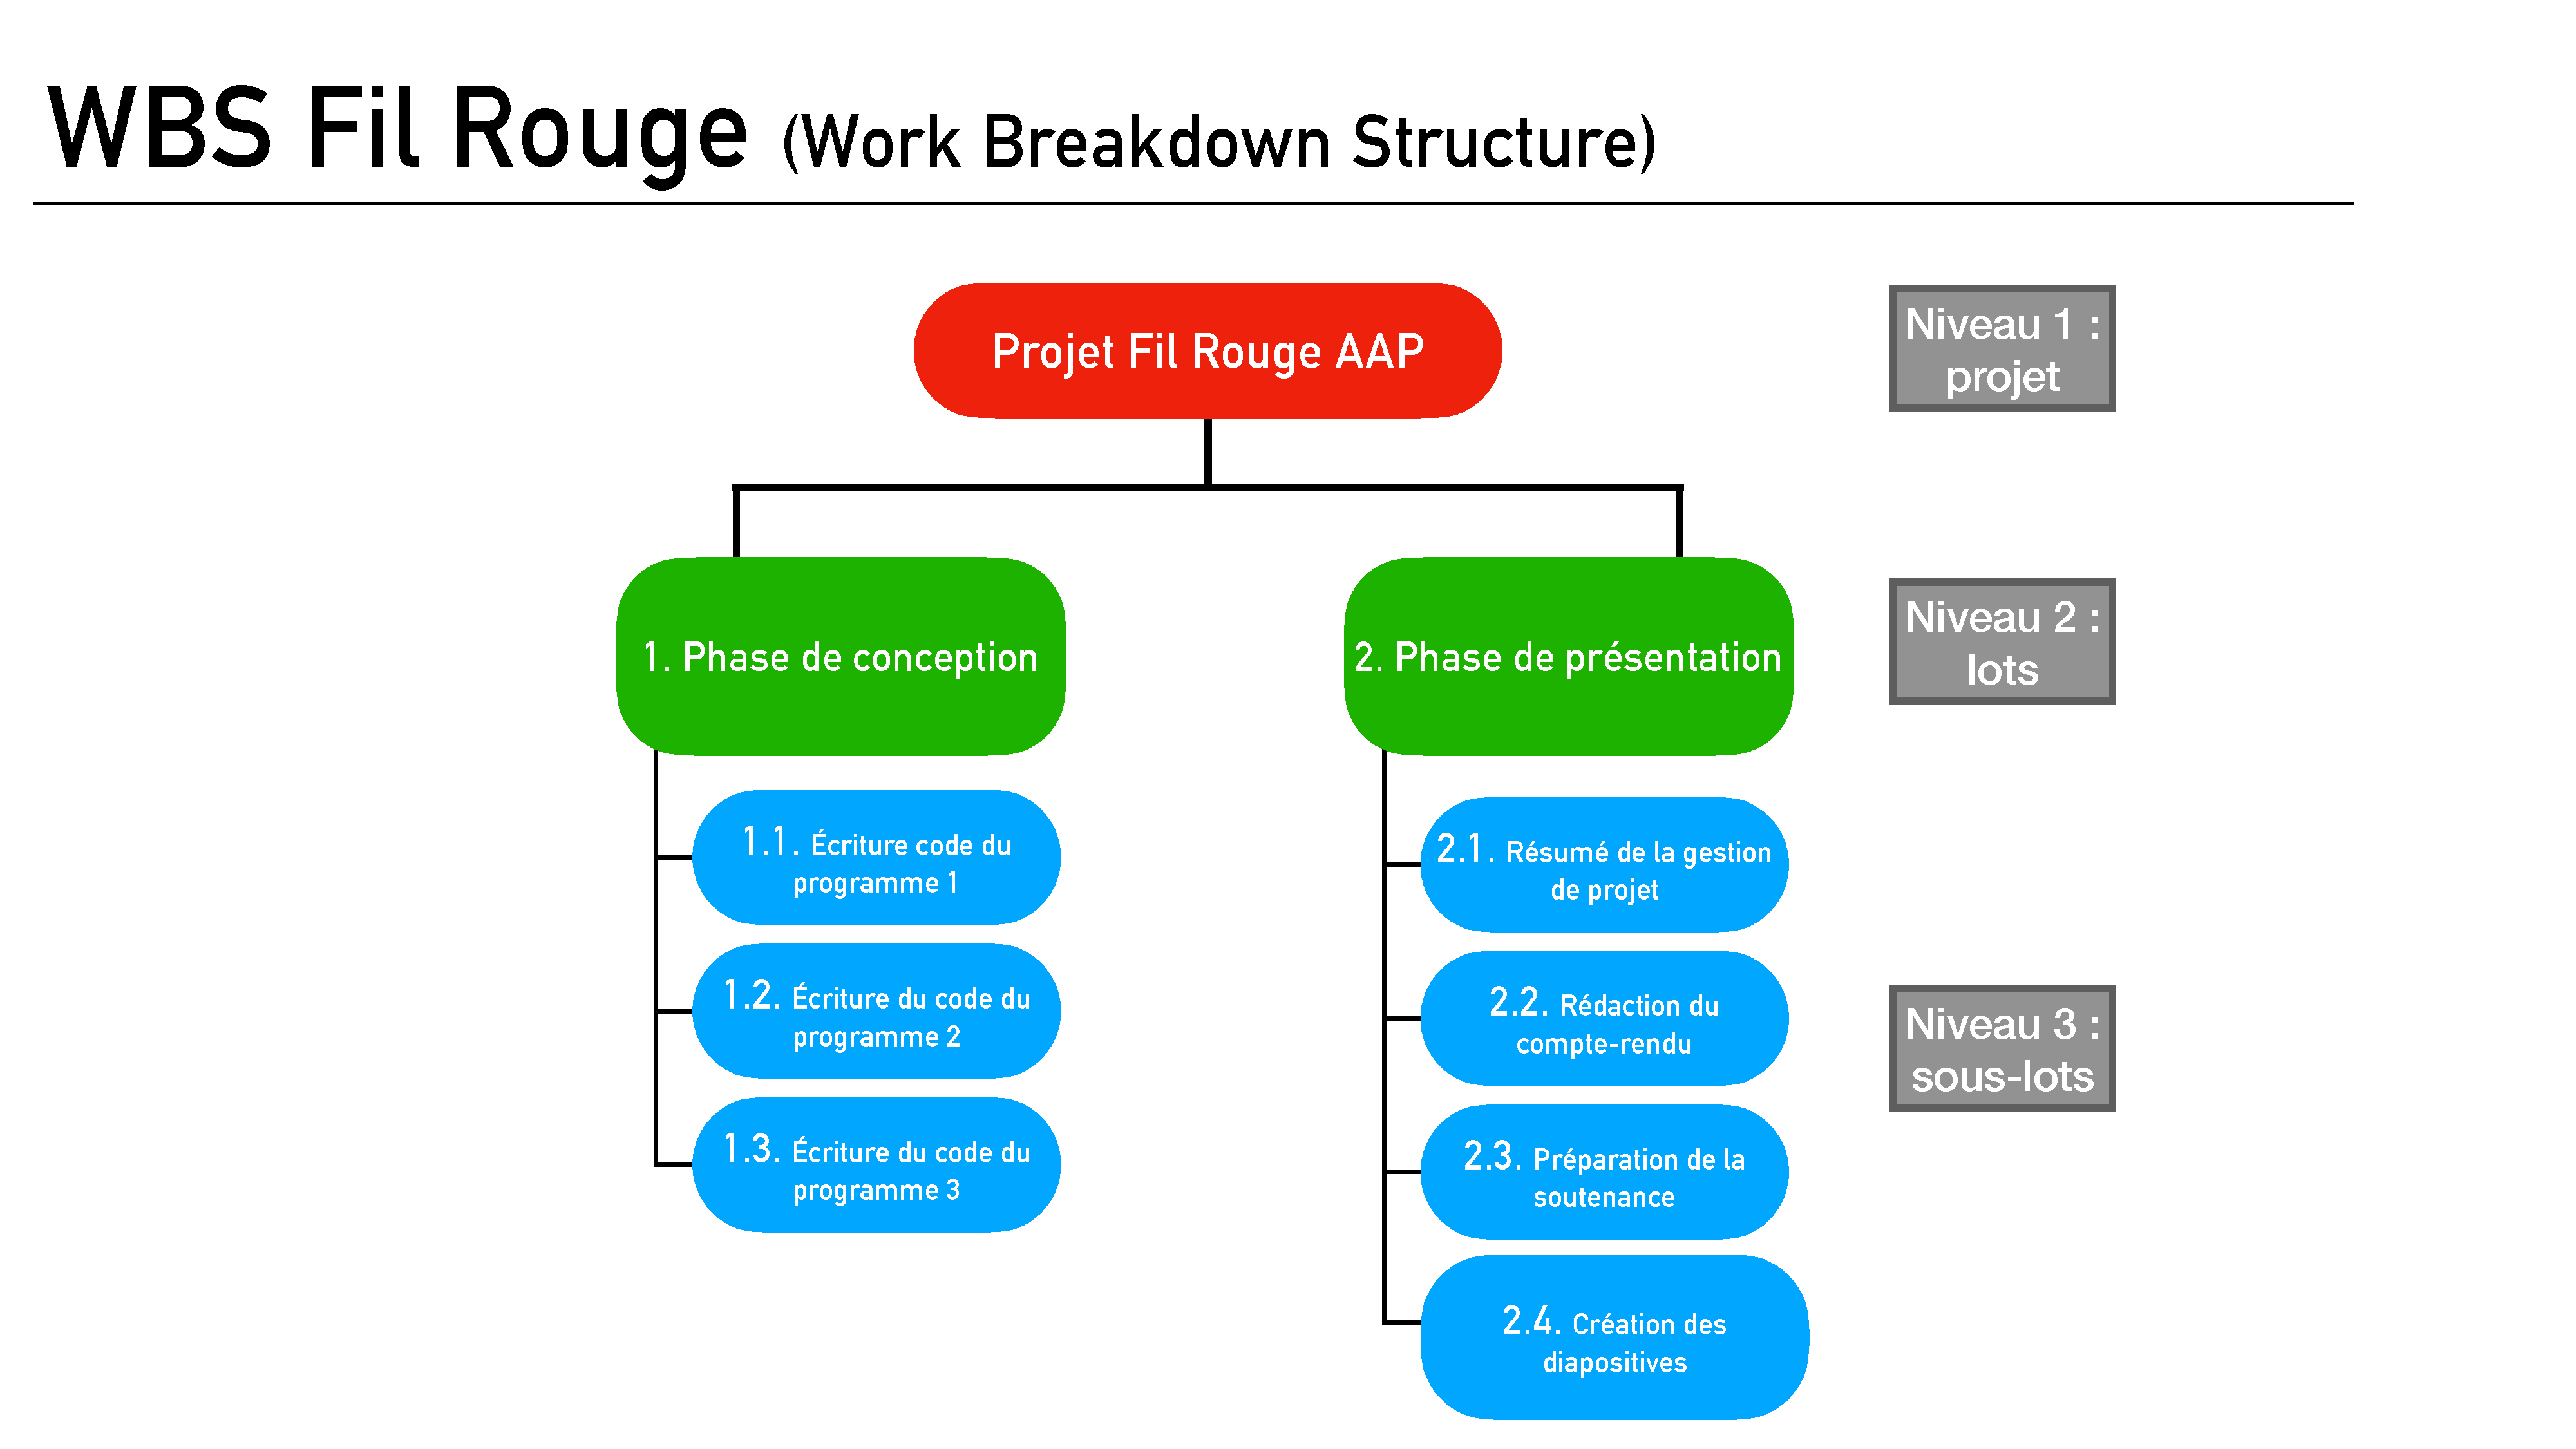
\includegraphics[scale=0.23]{Img_gdp/WBS.pdf}
  \end{center}
  \caption{Work Breakdown Structure- Fil rouge AAProximation}
  \label{fig:WBS}
\end{figure}


\begin{figure}[H]
  \begin{center}
    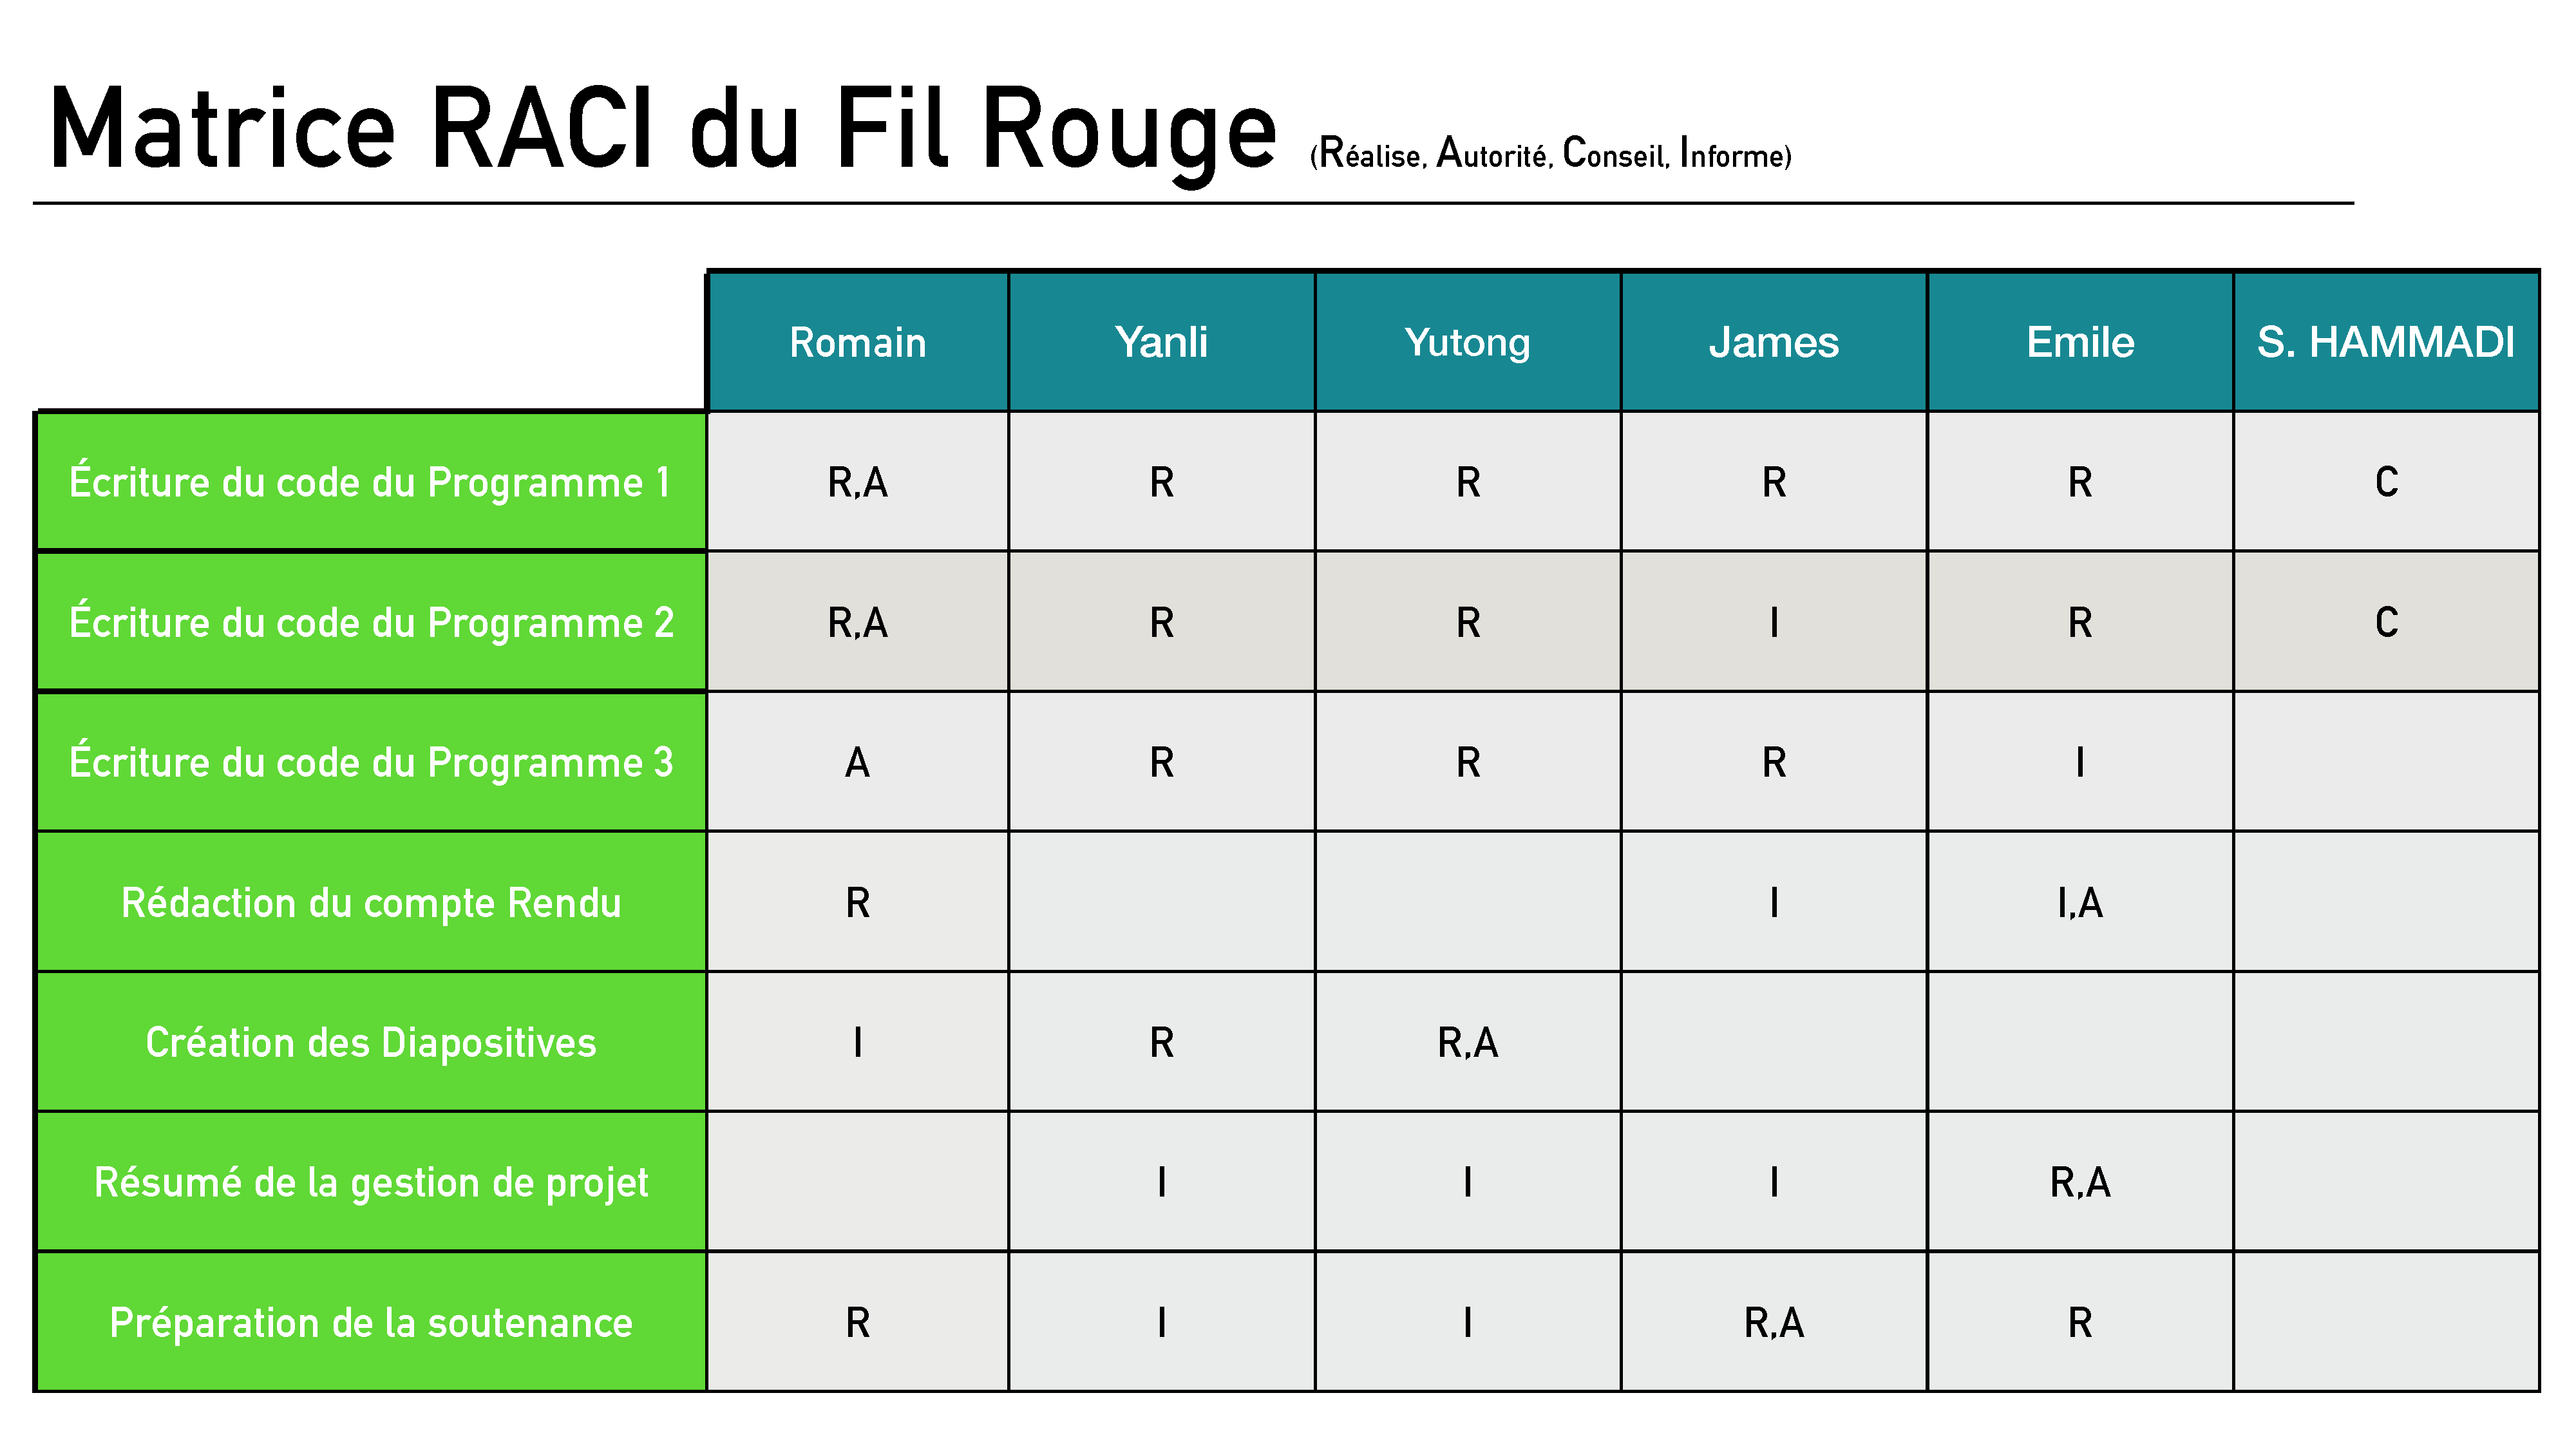
\includegraphics[scale=0.23]{Img_gdp/Matrice-RACI.pdf}
  \end{center}
  \caption{Matrice RACI - Fil rouge AAProximation}
  \label{fig:RACI}
\end{figure}




\section{Conclusion}

Pour conclure, nous pouvons dire que ce projet Fil Rouge a été formateur, il nous a permis de vraiment mieux se familiariser avec le language C et de réaliser un projet de nous même avec avec les différents aspect de la gestion de projet. Nous sommes ravi d’avoir pu faire ce projet, c’était l’occasion de travailler en groupe et de mettre en relation nos connaissances apprises durant ce cursus d'algorithme, ce qui a d’ailleurs considérablement approfondi nos connaissances sur le sujet. 



\nocite{*}

\bibliography{bibli}
\bibliographystyle{plain}

\vspace*{1cm}

\textbf{\LARGE Annexes : code des programmes}

\begin{appendix}
  \section{Code programme 1: \texttt{displayAVL.exe}}
  \lstinputlisting[language=C, lastline=179]{../Programme_1/avl.c}
  \vspace{1cm}
  \lstinputlisting[language=C]{../Programme_1/displayAVL.c}

  \section{Code programme 2: \texttt{indexation.exe}}
  \lstinputlisting{../Programme_2/indexation.c}

  \section{Code programme 3: \texttt{anagrammes.exe}}
  \lstinputlisting{../Programme_3/anagrammes.c}
\end{appendix}



\end{document}